% Two paths from -1 to 1: alpha along the upper unit semicircle, beta along
% the real diameter.
% Source: book/tex/complex-ana/holomorphic.tex (section: Cauchy-Goursat theorem).
\documentclass[border=2mm]{standalone}
\usepackage{tikz}
\usetikzlibrary{arrows.meta}
\begin{document}
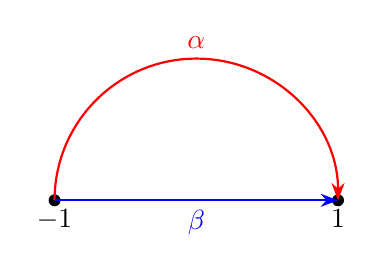
\begin{tikzpicture}[scale=1.8, >={Stealth[length=2.2mm]}]
  \fill (-1,0) circle (1.2pt) node[below] {$-1$};
  \fill (1,0) circle (1.2pt) node[below] {$1$};
  \draw[red, thick, ->] (180:1) arc (180:0:1);
  \node[red, above] at (90:1) {$\alpha$};
  \draw[blue, thick, ->] (-1,0) -- (1,0);
  \node[blue, below] at (0,0) {$\beta$};
\end{tikzpicture}
\end{document}
